%=====================================================================
%  How Much Domain Knowledge Does Cold-Start Energy Transfer Need?
%  IEEE conference style. Compiles on Overleaf (pdfLaTeX).
%  Self-contained: manual thebibliography, figures in ./figures/.
%=====================================================================
\documentclass[conference]{IEEEtran}
\IEEEoverridecommandlockouts

\usepackage{cite}
\usepackage{amsmath,amssymb,amsfonts}
\usepackage{bm}
\usepackage{graphicx}
\usepackage{booktabs}
\usepackage{array}
\usepackage{xcolor}
\usepackage{url}
\usepackage{tikz}
\usetikzlibrary{arrows.meta,positioning,fit,backgrounds}
\usepackage[colorlinks=true,allcolors=blue]{hyperref}

\let\proof\relax\let\endproof\relax % IEEEtran predefines these; let amsthm own them
\usepackage{amsthm}
\newtheorem{proposition}{Proposition}
\newcommand{\nrmse}{\mathrm{nRMSE}}
\newcommand{\thesource}{\mathcal{D}_{\mathrm{S}}}
\newcommand{\thetarget}{\mathcal{D}_{\mathrm{T}}}

\begin{document}

\title{How Much Domain Knowledge Does Cold-Start\\Energy Transfer Need?}

\author{\IEEEauthorblockN{Abdelhaq Dabaghia\IEEEauthorrefmark{1}}
\IEEEauthorblockA{\IEEEauthorrefmark{1}EnerTEF, Service~1 --- Energy Community Forecasting\\
Email: (corresponding author)}}

\maketitle

\begin{abstract}
When a data-scarce site must bootstrap an energy forecaster from a mature model at
another site, what actually limits the transfer --- the adaptation \emph{algorithm}
or the \emph{output representation}? We answer this on two real, published,
cross-site transfers with deployed industrial models: EV charging demand
(Luxembourg $\rightarrow$ UK \emph{Electric Nation}) and PV generation
(Luxembourg $\rightarrow$ a Konstanz household). First, we show the algorithm is
\emph{not} the lever: across the continual-learning (CL) taxonomy --- Elastic
Weight Consolidation (EWC) with source or target Fisher, MAS, LwF, DER++, A-GEM ---
\emph{no} method beats a plain warm-start on plasticity or simple replay on
retention; a scale-fairness control further shows the transferred Fisher's apparent
harm is a \emph{scale artifact}, not an intrinsic property. Second --- our main
contribution --- a \emph{controlled representation ablation}, holding architecture
and algorithm fixed and changing only how power is represented, moves warm-start
error by up to $8\times$, dwarfing any CL effect. Crucially, the \emph{best}
representation is task-dependent in a principled way: a generic reversible
per-instance normalisation (RevIN), the recent time-series SOTA, beats a
\emph{thin} domain representation (per-unit, a single capacity scalar) on EV
($\nrmse\,0.12$ vs.\ $0.27$, Wilcoxon $p{=}0.008$), but is itself beaten by a
\emph{rich} physical representation (the clear-sky index, an astronomical envelope)
on PV ($0.41$ vs.\ $0.65$, $p{=}0.008$). The value of a domain representation thus
scales with the structure it injects: cheap physics loses to learned per-instance
normalisation, rich physics beats it. A scale-decomposition analysis, whose
sufficient condition we verify on the deployed model, explains why scale-invariant
representations collapse the source/target Fisher mismatch (from ${\sim}122\times$
to ${\sim}1.5\times$); and a mechanistic study explains why replay beats EWC in
cross-regime transfer (the Fisher-important directions coincide with the useful
target gradients, $\cos{=}0.82$). We release a fully reproducible,
GPU-accelerated pipeline.
\end{abstract}

\begin{IEEEkeywords}
Transfer learning, representation, reversible instance normalisation, clear-sky
index, continual learning, catastrophic forgetting, EV charging demand, PV
generation, load forecasting.
\end{IEEEkeywords}

%=====================================================================
\section{Introduction}
%=====================================================================
Data-driven forecasters deployed in energy communities operate in
\emph{non-stationary} environments: consumption drifts, new assets appear, and new
sites must be served with little local history. When a fresh, data-scarce site
comes online, the practical recipe is \emph{transfer}: reuse a model trained on a
data-rich source and adapt it~\cite{PanYang2010}. A large literature then asks
\emph{how to adapt without forgetting} the source --- the province of continual
learning (CL) and its regularisers (EWC~\cite{Kirkpatrick2017}) and replay
buffers~\cite{Rolnick2019}. Our own production system (Service~1 of a Horizon
Europe project) does exactly this: a Luxembourg EV CNN--LSTM is nightly fine-tuned
with EWC.

This paper starts from a deployment-relevant question --- \emph{can a low-data
target bootstrap from the mature model, and keep adapting without forgetting?} ---
and arrives at a sharper one. We find that the CL \emph{algorithm} is essentially
irrelevant to the outcome, whereas the \emph{output representation} is decisive.
The contribution is therefore not another CL method but an answer to: \emph{what
property must a representation have for cross-site energy transfer, and how much
domain knowledge does it need to encode?}

Our answer is a controlled ablation on two physically distinct tasks. Holding the
deployed architecture and the transfer algorithm fixed, and changing \emph{only}
how power is represented, target error moves by up to $8\times$ --- more than any
CL intervention we could find. And the winner is task-dependent in a way that is
itself the message: a \emph{generic}, learned, per-instance normalisation (RevIN,
the recent time-series SOTA~\cite{RevIN2022}) beats a \emph{thin} domain-informed
representation (the power-engineering per-unit system, a single capacity scalar) on
EV, but a \emph{rich} physical representation (the solar clear-sky
index~\cite{Inman2013,Yang2018}) beats RevIN on PV. The value of injecting domain
knowledge scales with how much relevant structure it carries.

\noindent\textbf{Contributions.}
\begin{enumerate}
\item A \emph{controlled representation ablation} on two real cross-site transfers,
holding architecture and algorithm fixed and evaluating in physical units, that
isolates representation as the dominant lever (up to $8\times$ error range).
\item The main finding, significant on both tasks (Wilcoxon $p{=}0.008$): the best
representation depends on the \emph{richness} of the domain knowledge it encodes
--- learned per-instance normalisation (RevIN) beats \emph{thin} per-unit on EV,
but \emph{rich} clear-sky beats RevIN on PV.
\item A \emph{scale-decomposition} model (a proposition with a sufficient condition
we verify on the deployed model) that explains why scale-invariant representations
collapse the source/target Fisher mismatch.
\item A comprehensive \emph{negative result on CL algorithms} (EWC/MAS/LwF/DER++/
A-GEM never beat warm-start/replay), with a Fisher scale-fairness control and a
mechanistic explanation of why replay beats EWC in cross-regime transfer.
\item A fully reproducible, GPU-accelerated pipeline and a nine-country
distance$\rightarrow$transfer-gap analysis.
\end{enumerate}

%=====================================================================
\section{Related Work}
%=====================================================================
\textbf{Representation and normalisation for transfer.} Our central lever ---
the output representation --- connects three threads. (i)~\emph{Static, domain
representations}: the power-engineering \emph{per-unit} system normalises power by a
rated base~\cite{Glover}, and capacity/maximum normalisation into $[0,1]$ is
standard in load-forecasting transfer to make series building-agnostic before
fine-tuning~\cite{TLnorm}; in solar forecasting, the \emph{clear-sky index} (power
divided by a clear-sky model) de-seasonalises the diurnal/annual trend and is
widely reported to help regardless of model~\cite{Inman2013,Yang2018}.
(ii)~\emph{Learned, per-instance normalisation}: reversible instance normalisation
(RevIN)~\cite{RevIN2022} standardises each input window by its own statistics and
reverses this on the output, and has become a default for non-stationary
time-series forecasting; adaptive variants model evolving statistics (Dish-TS,
SAN, FAN)~\cite{DishTS2023,SAN2023,FAN2024}. Recent work debates whether the RevIN
affine layer is even needed~\cite{RevINrole2026}. \emph{Our contribution is not any
one of these normalisations but a head-to-head, controlled comparison across all
three families on real cross-site transfer, and the finding that the winner is
governed by the richness of the domain structure injected.}

\textbf{Continual learning} splits into~\cite{DeLange2021}
\emph{regularisation} (EWC~\cite{Kirkpatrick2017},
SI~\cite{Zenke2017}, MAS~\cite{Aljundi2018}, LwF~\cite{LiHoiem2017}),
\emph{replay} (iCaRL~\cite{Rebuffi2017}, ER~\cite{Rolnick2019},
DER++~\cite{Buzzega2020}), and \emph{parameter isolation}; online EWC variants keep
a running Fisher~\cite{Schwarz2018}. CL is increasingly applied to load/building
energy forecasting under drift~\cite{ContLoadPartsCleaning2025,BuildingEnergyCL2023,
OODLoadCovid2023,PracticalCLEnergy2026,CLTimeSeriesSurvey2024}, and transfer for
EV/charging demand is motivated by data scarcity at new
sites~\cite{EVTransferGaps2025,EVScarceCluster2025}. We contribute a rigorous
negative result on this taxonomy for cross-site cold-start.

\textbf{Gap.} Prior CL/transfer forecasting studies typically use synthetic splits
or a single method, and rarely (a)~validate on an \emph{independent published}
target, (b)~compare \emph{representations} against the per-instance-normalisation
SOTA under a fixed architecture, or (c)~ask what representation \emph{property}
drives transfer. We address all three.

%=====================================================================
\section{Problem Setup and Data}
%=====================================================================
\subsection{Tasks and domains}
We study two deployed forecasters and two real, published, independent targets.
\textbf{EV demand:} source $\thesource$ is the Luxembourg production domain
(aggregated EV charging power, two chargers, $15$-min, 2024-09-10 to 2026-01-18,
$47{,}524$ steps); target $\thetarget$ is the UK \emph{Electric Nation}
smart-charging trial (${\sim}72$ home chargers, Amps$\to$kW at $230$\,V,
2017-06-28 to 2018-12-16, $51{,}467$ steps). \textbf{PV generation:} source is the
Luxembourg community PV; target is household \texttt{DE\_KN\_residential3} of the
OPSD dataset~\cite{OPSD2020} (Konstanz, Germany), a $15$-min series over
2016--2018. Weather is from the Open-Meteo archive. Both transfers are dominated by
a large \emph{scale} gap ($6\times$ demand for EV, $50\times$ capacity for PV) while
weather transfers well (standardised weather MMD$^2\!=\!0.034$/$0.027$
respectively~\cite{Gretton2012}), Table~\ref{tab:domain}.

\begin{table}[t]
\centering
\caption{Domain shift (EV: LU vs.\ UK). $W_{\mathrm{norm}}$ is the $1$-Wasserstein
distance on pooled-std-normalised marginals. The shift is dominated by demand scale.}
\label{tab:domain}
\begin{tabular}{lccc}
\toprule
Variable & $W_{\mathrm{norm}}$ & LU (mean$\pm$std) & UK (mean$\pm$std)\\
\midrule
\texttt{ev\_kw}      & \textbf{0.62} & $40.7\pm66.5$ & $16.8\pm15.2$\\
shortwave rad.       & 0.05 & $124\pm202$ & $122\pm189$\\
temperature          & 0.23 & $10.6\pm7.3$& $11.2\pm5.9$\\
wind speed           & \textbf{0.63} & $10.9\pm6.1$& $15.6\pm7.8$\\
\midrule
\multicolumn{4}{l}{weather MMD$^2=0.034$ \quad ev\_kw scale ratio $=6\times$}\\
\bottomrule
\end{tabular}
\end{table}

\subsection{Architectures and features}
We reproduce both deployed models to machine precision ($\max|\Delta|{=}0$) for
weight transfer. The \textbf{EV} model is a two-branch CNN--LSTM: a $(672,21)$
lookback through two causal \texttt{Conv1D}$(64,k5)$ and an \texttt{LSTM}$(64)$; a
$(20)$ next-step exogenous vector through \texttt{Dense}$(64)$; concatenated into
\texttt{Dense}$(128)\!\to\!\texttt{Dense}(1)$, Huber ($\delta{=}0.5$).
The \textbf{PV} model is a stacked LSTM ($96$ lookback, $11$ features, $148{,}161$
params). Features are the production sets (EV: \texttt{ev\_kw}, lags $\{1,4,96,672\}$,
rolling means, six weather, cyclic time; PV: \texttt{pv\_kw}, six weather, cyclic
time). We reuse the frozen production scalers for the CL study; the representation
ablation replaces the power normalisation as described in Sec.~\ref{sec:reps}.

\subsection{Cold-start transfer protocol and metrics}
Let $\theta^{\star}$ be the transferred production weights. Conditions:
\emph{B0} from scratch; \emph{B3} warm-start plain fine-tune;
\emph{B1/B4} warm-start$+$EWC (source/target Fisher); \emph{B5} warm-start$+$replay.
Only the first $N$ days of the target stream are used for training; evaluation is on
a fixed final $14$-day holdout. Plasticity is target
$\nrmse=\mathrm{RMSE}/\overline{y}$ in physical units (kW); stability is the
\emph{source-retention} $\nrmse$ of the adapted model on a fixed source holdout.
All comparisons use paired Wilcoxon signed-rank tests over seeds.

%=====================================================================
\section{Representation Governs Transfer}
\label{sec:reps}
%=====================================================================
This is the paper's core. We fix the architecture, the algorithm (plain warm-start
B3 vs.\ from-scratch B0), the data budget ($N{=}30$), and the exogenous inputs, and
vary \emph{only} how the power channel and the target are represented. Because each
representation changes the target space, the frozen production weights no longer
apply; we train a source model \emph{from scratch} in each representation and
transfer it, a self-contained test. All errors are reported back in kW.

\subsection{The representations}
We compare three families (min--max scaling is excluded: source-fit min--max places
the target in a tiny sub-range and is uniformly the worst, a known
pathology we do not belabour):
\begin{itemize}
\item \textbf{Static global} (source-fit): \emph{z-score}, \emph{robust}
(median/IQR), and \emph{log} (variance-stabilising).
\item \textbf{Learned per-instance} (the SOTA family): \emph{RevIN} --- we use the
affine-free form, standardising the power channel by the lookback mean/std of each
window and de-normalising the prediction with the same statistics (we drop the
affine layer, whose necessity is contested~\cite{RevINrole2026}).
\item \textbf{Domain-informed}: \emph{per-unit} for EV (divide each site's power by
its own capacity --- a single scalar) and the \emph{clear-sky index} for PV
(power divided by an astronomical envelope, the $95$th power percentile per
$(10$-day$)\times($time-of-day$)$ bin, fit on training rows only --- a rich
per-timestamp structure).
\end{itemize}
We also implemented a SAN-style~\cite{SAN2023} slice normalisation, but our
reimplementation was not competitive and we omit it rather than present a
strawman; a faithful comparison to adaptive-normalisation methods
(SAN/Dish-TS/FAN) is left to future work.

\subsection{Main result: the winner depends on domain-knowledge richness}
Table~\ref{tab:ablation} is the central result. Two facts stand out.

\emph{(1) Representation is the dominant lever.} Within a task, the best and worst
representations differ by up to $8\times$ in warm-start error --- with the
architecture and algorithm held fixed. No CL intervention we test
(Sec.~\ref{sec:cl}) comes close to this range. Notably, global affine centring
(z-score, robust) is not merely suboptimal but \emph{actively harmful for PV}: the
day/night bimodal distribution and frequent zeros make the de-normalised
predictions diverge (Table~\ref{tab:ablation}, ``diverges'').

\emph{(2) The winner is task-dependent, by richness.} On EV, \textbf{RevIN wins}
($\nrmse\,0.116$), beating the thin per-unit representation ($0.273$) and all global
scalers, significantly (paired Wilcoxon, $8$ seeds, RevIN vs.\ per-unit
$p{=}0.008$; vs.\ robust/z-score $p{=}0.008$). On PV, \textbf{clear-sky wins}
($0.409$), beating RevIN ($0.645$) and log ($0.661$), significantly (clear-sky vs.\
RevIN $p{=}0.008$; vs.\ log $p{=}0.008$). The difference between the two tasks is
the \emph{amount of structure} the domain representation encodes: per-unit injects a
single capacity scalar and loses to a generic learned per-instance normaliser;
clear-sky injects a full astronomical envelope and beats it.

\begin{table}[t]
\centering
\caption{Representation ablation: warm-start (B3) target $\nrmse$ at $N{=}30$
(mean$\pm$std, $8$ seeds; $^\dagger$ log-EV at $5$ seeds). Architecture and
algorithm are fixed; only the power representation changes. \textbf{Bold} = per-task
winner. The domain-informed row is per-unit for EV and clear-sky for PV.}
\label{tab:ablation}
\begin{tabular}{lcc}
\toprule
Representation (family) & EV $\nrmse$ & PV $\nrmse$\\
\midrule
z-score (global)                 & $0.295\pm.014$ & diverges\\
robust (global)                  & $0.282\pm.017$ & diverges\\
log (global)                     & $0.424\pm.013^\dagger$ & $0.661\pm.065$\\
RevIN (learned per-instance)     & $\mathbf{0.116\pm.003}$ & $0.645\pm.019$\\
domain-informed (per-unit / csi) & $0.273\pm.010$ & $\mathbf{0.409\pm.013}$\\
\midrule
per-task winner                  & RevIN & clear-sky\\
Wilcoxon (winner vs.\ 2nd)       & $p{=}0.008$ & $p{=}0.008$\\
\bottomrule
\end{tabular}
\end{table}

\noindent\textbf{Robustness (not a re-training artefact).} On EV, applying per-unit
directly to the \emph{deployed} production model with no re-training (the target is
simply rescaled to its own per-unit base) still cuts transfer error from $0.51$ to
$0.39$ ($3$ seeds), confirming the representation effect is genuine and not an
artefact of re-fitting the source.

\noindent\textbf{Takeaway.} The most effective ``continual-learning'' intervention
here is not an algorithm but a change of representation. A learned, reversible
per-instance normalisation is a very strong \emph{default} --- it neutralises
cross-site scale \emph{and} local non-stationarity generically --- and is beaten
only by a domain representation that injects sufficiently rich physical structure.

%---------------------------------------------------------------------
\subsection{Why scale-invariance helps: a scale-decomposition model}
\label{sec:scale-model}
Every winning representation is at least scale-invariant. We formalise why, via the
source/target importance mismatch. Let $\Omega_d\in\mathbb{R}_{+}^{p}$ be the
diagonal Fisher-importance vector at site $d$ and $S(\Omega_d)=\tfrac1p\sum_j
\Omega_{d,j}$ its mean. Working in logs makes scale factors additive; we use the
symmetric log-mismatch
\begin{equation}
M(\Omega_s,\Omega_t)=\bigl|\log S(\Omega_s)-\log S(\Omega_t)\bigr|.
\label{eq:logmismatch}
\end{equation}
Assume only a multiplicative scale model (the exponent left unspecified),
$S(\Omega_d^{\mathrm{raw}})=c_d\,S(\Omega_d^{\mathrm{struct}})$, with $c_d>0$ a
site-dependent nuisance factor. We do \emph{not} claim normalisation
unconditionally reduces mismatch (it can change trajectories, representations and
gradients); a useful result must be conditional.

\begin{proposition}[Scale-aligned mismatch reduction]
\label{prop:scale}
Write $A_{s,t}=\log(c_s/c_t)$ (nuisance discrepancy) and
$R_{s,t}=\log\!\bigl(S(\Omega_s^{\mathrm{struct}})/S(\Omega_t^{\mathrm{struct}})\bigr)$
(structural residual); under the scale model, $M_{\mathrm{raw}}=|A_{s,t}+R_{s,t}|$
and $M_{\mathrm{norm}}=|R_{s,t}|$. If the two share sign, $A_{s,t}R_{s,t}\ge0$, then
$M_{\mathrm{norm}}\le M_{\mathrm{raw}}$, strictly if $A_{s,t}\neq0$.
\end{proposition}
\begin{proof}
When $A_{s,t}R_{s,t}\ge0$ the terms share sign (or one is zero), so
$|A_{s,t}+R_{s,t}|=|A_{s,t}|+|R_{s,t}|\ge|R_{s,t}|=M_{\mathrm{norm}}$.
\end{proof}

For separately trained models a residual $E_{s,t}$ (retraining, estimation noise)
is added, giving the robust sufficient condition $A_{s,t}R_{s,t}\ge0$ and
$|E_{s,t}|<|A_{s,t}|$. \textbf{We verify this directly}, with no retraining, on the
deployed EV model: $A_{s,t}{=}{+}4.40{\pm}0.12$ and $R_{s,t}{=}{+}0.40{\pm}0.06$
(both positive, the sign condition holds on \emph{every} seed), collapsing the
mismatch from $M_{\mathrm{raw}}{=}4.80$ ($\sim$$122\times$) to $M_{\mathrm{norm}}
{=}0.40$ ($\sim$$1.5\times$). Two honesty notes: the reduction is a consequence of a
\emph{verified} condition, not an assumption; and $R_{s,t}>0$ shows a genuine
residual structural difference survives --- scale-invariance removes the scale
nuisance, not all cross-site mismatch, which is exactly why a \emph{rich} domain
representation (clear-sky) can still add value beyond a scale-free normaliser.

%=====================================================================
\section{The Algorithm Is Not the Lever}
\label{sec:cl}
%=====================================================================
We now show the complementary half: no CL algorithm delivers anything like the
representation effect. All runs: Adam ($10^{-4}$), $10$ epochs, batch $64$; RTX~5070
(TensorFlow~$2.21$/CUDA~$12.9$, WSL2).

\subsection{Warm-start helps; EWC does not; replay wins retention}
Warm-start cuts target $\nrmse$ by ${\sim}40\%$ vs.\ from-scratch at every budget
$N\!\in\!\{1,7,30,60,90\}$ (Fig.~\ref{fig:rq1}). At $N{=}30$ over $8$ seeds
(Table~\ref{tab:rq2}), \textbf{EWC (B4) is statistically indistinguishable from a
plain warm-start on plasticity} ($p{=}0.31$), while \textbf{replay (B5)
significantly improves source retention} ($p{=}0.008$) at a significant plasticity
cost ($p{=}0.008$). EWC buys neither axis.

\begin{figure}[t]
\centering
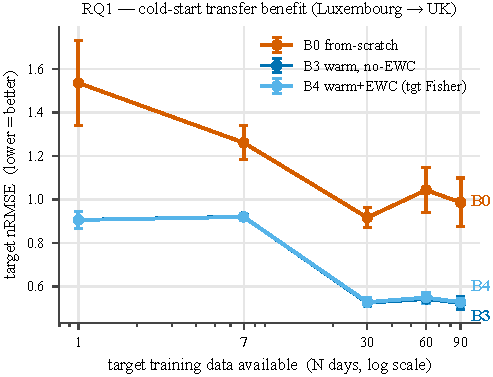
\includegraphics[width=0.92\linewidth]{figures/fig_rq1_coldstart.pdf}
\caption{Warm-start (B3/B4) vs.\ from-scratch (B0): target $\nrmse$ vs.\ target
data $N$ (mean$\pm$std). Warm-start helps at every budget; EWC (B4) tracks B3.}
\label{fig:rq1}
\end{figure}

\begin{table}[t]
\centering
\caption{Stability--plasticity at $N{=}30$ (mean$\pm$std, $8$ seeds).}
\label{tab:rq2}
\begin{tabular}{lcc}
\toprule
Condition & target $\nrmse$ & source-retention $\nrmse$\\
\midrule
B0 from-scratch          & $1.06\pm.16$ & $1.54\pm.09$\\
B3 warm, no-EWC          & $\mathbf{0.52\pm.02}$ & $0.56\pm.03$\\
B1 warm+EWC (src Fisher) & $0.77\pm.01$ & $0.62\pm.01$\\
B4 warm+EWC (tgt Fisher) & $0.52\pm.02$ & $0.56\pm.03$\\
B5 warm+replay           & $0.71\pm.02$ & $\mathbf{0.43\pm.03}$\\
\bottomrule
\end{tabular}
\end{table}

\subsection{The transferred Fisher's harm is a scale artifact}
Naively B1 (source Fisher) looks far worse than B4 (target Fisher). But the source
Fisher's raw scale is ${\sim}211\times$ larger --- a direct consequence of the
$6\times$ demand-scale gap propagating through the output-sensitivity Fisher --- so
at a shared $\lambda$ it over-regularises. Normalising each Fisher to unit mean and
sweeping $\lambda$ makes B1 and B4 comparable and \emph{neither} beats warm-start:
the Fisher's \emph{origin} does not matter once scales are equalised. This ties
directly to Sec.~\ref{sec:scale-model}: the same scale nuisance that per-unit
removes is what made the transferred Fisher look harmful.

\subsection{The full CL taxonomy fails too}
To rule out that a different family would win, we bench the standard taxonomy at
$N{=}30$ (Table~\ref{tab:clsuite}): MAS, LwF, DER++, A-GEM, plus improved-EWC
variants (true empirical Fisher, per-layer normalisation, EWC$+$replay hybrid) and a
learning-rate/epoch sweep. \textbf{None beats warm-start on plasticity or replay on
retention.} The PV task reaches the same verdict, confirming the conclusion is not
EV-specific.

\begin{table}[t]
\centering
\caption{CL taxonomy (EV, $N{=}30$). No method beats warm-start on plasticity or
replay on retention.}
\label{tab:clsuite}
\begin{tabular}{llcc}
\toprule
Method & Family & target $\nrmse$ & retention $\nrmse$\\
\midrule
B3 warm    & (reference)        & $\mathbf{0.52}$ & $0.56$\\
B5 replay  & (reference)        & $0.68$ & $\mathbf{0.40}$\\
MAS        & regularisation     & $0.82$ & $0.58$\\
LwF        & distillation       & $0.68$ & $0.58$\\
DER++      & replay$+$distill   & $0.78$ & $0.62$\\
A-GEM      & replay$+$projection& $0.55$ & $0.55$\\
EWC (best variant) & regularisation & $0.76$ & $0.53$\\
\bottomrule
\end{tabular}
\end{table}

\subsection{Why replay beats EWC: a mechanism}
\label{sec:mech}
We explain \emph{why} regularisation fails in cross-regime transfer, with probes at
$\theta^{\star}$ (EV, $N{=}30$). \textbf{(b)~The Fisher-important directions
coincide with the useful target gradients}: $\cos(F,|g|){=}0.82$, and $62\%$ of the
target-gradient energy lies in the top-decile Fisher directions (vs.\ $10\%$ if
unrelated) --- source and target share the \emph{task} but differ in \emph{regime},
so the parameters that matter for the source are exactly those the target must move.
\textbf{(a)~EWC steers motion away from these directions}: it moves the weights a
similar distance to a plain fine-tune yet its target error barely falls, buying
neither plasticity nor retention. \textbf{(c)~Replay works by coverage}: source
retention improves only once the buffer covers the source distribution ($0.50$ at
$50$ samples $\to0.39$ at ${\ge}10^3$), a concrete memory budget. Together:
regularising toward $\theta^{\star}$ fights exactly the updates the target needs,
while replay supplies the source objective directly.

%=====================================================================
\section{Domain Distance and the Transfer Gap}
%=====================================================================
Across \emph{nine} countries' real national solar generation (OPSD, 2018--2019),
transferring the per-unit Luxembourg PV source, the transfer gap grows with the
source$\rightarrow$target generation-shape distance ($\rho{=}0.88$, $p{=}0.004$;
Fig.~\ref{fig:multi}). \emph{However}, this is largely \textbf{mediated by the
target's intrinsic predictability}: a model-free climatology baseline explains
$94\%$ of the warm-start-error variance ($r{=}0.94$) and is collinear with distance.
Domain distance is thus a useful \emph{predictor} of the transfer gap --- rarely
established on real, geographically diverse targets --- but acts mostly through
intrinsic target difficulty, not a pure distance penalty.

\begin{figure}[t]
\centering
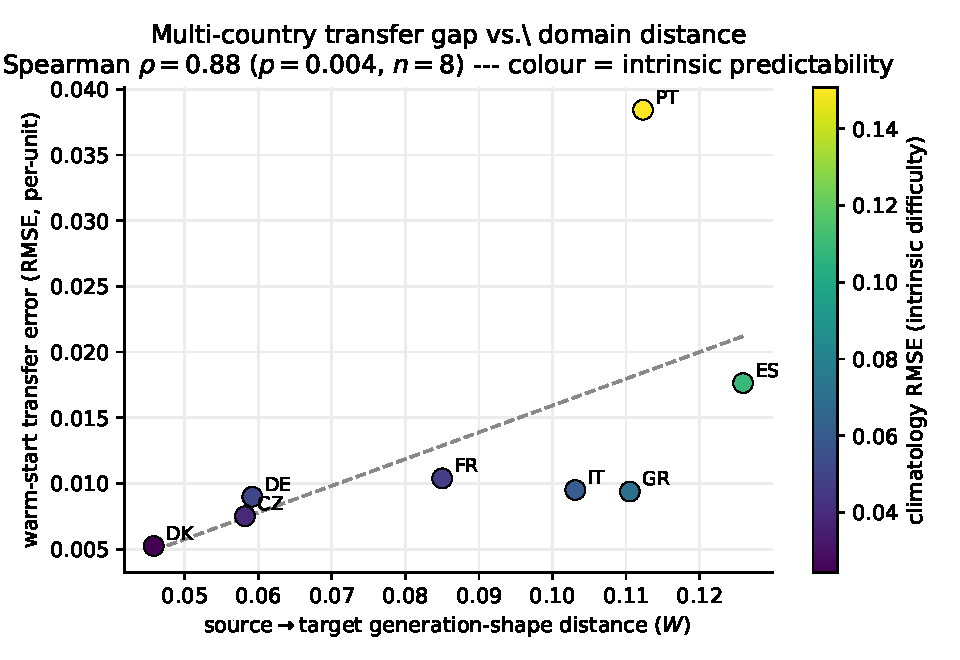
\includegraphics[width=0.92\linewidth]{figures/fig_multicountry.pdf}
\caption{Across nine countries, warm-start error grows with generation-shape
distance ($\rho{=}0.88$), but colour (climatology error = intrinsic difficulty)
shows the trend is largely mediated by target predictability.}
\label{fig:multi}
\end{figure}

%=====================================================================
\section{Discussion}
%=====================================================================
The practical message reverses the usual emphasis. For cross-site cold-start energy
transfer, effort is better spent on the \emph{representation} than on the adaptation
algorithm. A learned reversible per-instance normalisation (RevIN) is a strong,
cheap default that should be the baseline for any such transfer --- it beat a
deployed domain convention (per-unit) outright on EV. Yet it is not the ceiling:
where a rich physical model of the signal exists (clear-sky for PV), encoding it
beats the generic normaliser. The design rule is to prefer the representation that
neutralises the most \emph{relevant} non-stationarity: generic per-instance scaling
when no rich structure is available, domain physics when it is. For adaptation,
prefer warm-start plus a small replay buffer over EWC.

%=====================================================================
\section{Limitations}
%=====================================================================
(1)~\emph{Diversity}: two tasks and, for PV, one primary target plus nine
cross-country sites; the ``RevIN vs.\ domain'' crossover is established on these two
tasks and should be tested more widely. (2)~\emph{Run-to-run variance}: GPU
non-determinism (cuDNN LSTM) induces cross-run variability, notably on PV; we
therefore rely on paired Wilcoxon tests over $8$ seeds and report the ranking and
significance, not the exact decimals, as the robust claims. (3)~\emph{Adaptive-norm
baselines}: we compare to RevIN but leave a faithful SAN/Dish-TS/FAN comparison to
future work. (4)~\emph{Weather approximations} and the fact that the UK data
reflects a smart-charging trial intervention. (5)~Absolute error remains high on EV
(large demand shift); the benefit is relative to from-scratch.

%=====================================================================
\section{Conclusion}
%=====================================================================
On two real cross-site cold-start transfers, the output representation --- not the
continual-learning algorithm --- governs transfer, moving error by up to $8\times$
while no CL variant beats warm-start$+$replay. Among representations, the winner
depends on the richness of the domain knowledge encoded: a generic learned
per-instance normalisation (RevIN) beats a thin domain representation (per-unit) on
EV, but a rich physical one (clear-sky) beats RevIN on PV --- both at $p{=}0.008$. A
scale-decomposition analysis, verified on the deployed model, explains why
scale-invariant representations collapse the source/target importance mismatch, and
a mechanistic study explains why replay beats EWC. We release a fully reproducible
pipeline.

%=====================================================================
\section*{Reproducibility}
%=====================================================================
Model builders (verified to $\max|\Delta|{=}0$), windowing, Fisher estimators, the
parameterised B0--B5 trainer, the representation-ablation drivers (EV and PV, with
incremental/resume logging), per-run CSV logs, seeds, and figures are released. GPU
runs use \texttt{tensorflow[and-cuda]} under WSL2.

%=====================================================================
\begin{thebibliography}{99}
\bibitem{PanYang2010} S.~J.~Pan and Q.~Yang, ``A survey on transfer learning,''
\emph{IEEE TKDE}, vol.~22, no.~10, pp.~1345--1359, 2010.
\bibitem{Kirkpatrick2017} J.~Kirkpatrick \emph{et al.}, ``Overcoming catastrophic
forgetting in neural networks,'' \emph{PNAS}, vol.~114, no.~13, pp.~3521--3526, 2017.
\bibitem{Rolnick2019} D.~Rolnick \emph{et al.}, ``Experience replay for continual
learning,'' in \emph{NeurIPS}, 2019.
\bibitem{RevIN2022} T.~Kim \emph{et al.}, ``Reversible instance normalization for
accurate time-series forecasting against distribution shift,'' in \emph{ICLR}, 2022.
\bibitem{DishTS2023} W.~Fan \emph{et al.}, ``Dish-TS: A general paradigm for
alleviating distribution shift in time series forecasting,'' in \emph{AAAI}, 2023.
\bibitem{SAN2023} Z.~Liu \emph{et al.}, ``Adaptive normalization for non-stationary
time series forecasting: A temporal slice perspective,'' in \emph{NeurIPS}, 2023.
\bibitem{FAN2024} W.~Ye \emph{et al.}, ``Frequency adaptive normalization for
non-stationary time series forecasting,'' in \emph{NeurIPS}, 2024.
\bibitem{RevINrole2026} ``On the role of reversible instance normalization in time
series forecasting,'' arXiv, 2026.
\bibitem{DeLange2021} M.~De~Lange \emph{et al.}, ``A continual learning survey,''
\emph{IEEE TPAMI}, vol.~44, no.~7, pp.~3366--3385, 2021.
\bibitem{Zenke2017} F.~Zenke, B.~Poole, and S.~Ganguli, ``Continual learning
through synaptic intelligence,'' in \emph{ICML}, 2017.
\bibitem{Aljundi2018} R.~Aljundi \emph{et al.}, ``Memory aware synapses,'' in
\emph{ECCV}, 2018.
\bibitem{LiHoiem2017} Z.~Li and D.~Hoiem, ``Learning without forgetting,''
\emph{IEEE TPAMI}, vol.~40, no.~12, pp.~2935--2947, 2017.
\bibitem{Rebuffi2017} S.-A.~Rebuffi \emph{et al.}, ``iCaRL,'' in \emph{CVPR}, 2017.
\bibitem{Buzzega2020} P.~Buzzega \emph{et al.}, ``Dark experience for general
continual learning,'' in \emph{NeurIPS}, 2020.
\bibitem{Schwarz2018} J.~Schwarz \emph{et al.}, ``Progress \& compress,'' in
\emph{ICML}, 2018.
\bibitem{CLTimeSeriesSurvey2024} Q.~Besnard \emph{et al.}, ``Continual learning for
time series forecasting: A first survey,'' 2024.
\bibitem{ContLoadPartsCleaning2025} ``Continual learning for very short-term load
forecasting,'' \emph{Applied Energy}, vol.~402, 2025.
\bibitem{BuildingEnergyCL2023} ``Comparison and demonstration of continual learning
for adaptive building energy prediction,'' \emph{Applied Energy}, 2023.
\bibitem{OODLoadCovid2023} ``Navigating out-of-distribution electricity load
forecasting during COVID-19,'' arXiv:2309.04296, 2023.
\bibitem{PracticalCLEnergy2026} ``Towards continuous power forecasting: Practical
continual learning for real-world energy systems,'' arXiv:2606.24955, 2026.
\bibitem{EVTransferGaps2025} ``Bridging data gaps for EV demand estimation: A
transfer learning approach,'' \emph{J.\ Transport Geography}, 2025.
\bibitem{EVScarceCluster2025} ``Enhancing EV charging load prediction in
data-scarce scenarios,'' \emph{Energy \& AI}, 2025.
\bibitem{Gretton2012} A.~Gretton \emph{et al.}, ``A kernel two-sample test,''
\emph{JMLR}, vol.~13, pp.~723--773, 2012.
\bibitem{OPSD2020} Open Power System Data, ``Household data,'' 2020. [Online].
Available: \url{https://data.open-power-system-data.org/household_data/}
\bibitem{Glover} J.~D.~Glover, M.~S.~Sarma, and T.~J.~Overbye, \emph{Power System
Analysis and Design}. Cengage Learning.
\bibitem{TLnorm} ``Energy predictive models with limited data using transfer
learning,'' arXiv:1906.02646, 2019.
\bibitem{Inman2013} R.~H.~Inman, H.~T.~C.~Pedro, and C.~F.~M.~Coimbra, ``Solar
forecasting methods for renewable energy integration,'' \emph{Prog.\ Energy
Combust.\ Sci.}, vol.~39, no.~6, pp.~535--576, 2013.
\bibitem{Yang2018} D.~Yang \emph{et al.}, ``History and trends in solar irradiance
and PV power forecasting,'' \emph{Solar Energy}, vol.~168, pp.~60--101, 2018.
\end{thebibliography}

\end{document}
